\documentclass{article}

\usepackage{isabelle,isabellesym}
\usepackage{url}
\usepackage{graphicx}
\usepackage{wrapfig}
\usepackage{placeins}

\usepackage{amssymb}

\usepackage[english]{babel}

\usepackage{booktabs}

\newcommand{\titl}{Verified Synthesis of Knowledge-Based Programs in Finite Synchronous Environments}
\newcommand{\stitl}{Knowledge-Based Programs}
\newcommand{\atitl}{\titl: \stitl}

\usepackage{color}
\definecolor{lcol}{rgb}{0,0,0}
%% \usepackage[a4paper,bookmarks=false,
%%             colorlinks=true,linkcolor=lcol,citecolor=lcol,
%%             filecolor=lcol,pagecolor=lcol,urlcolor=lcol,
%%             pdfauthor={Peter Gammie},
%%             pdftitle={\atitl},
%%             plainpages=false]{hyperref}

\newcommand{\isafun}[1]{{\sf #1}}

\renewcommand{\isastyletxt}{\isastyletext}
\renewcommand{\isadigit}[1]{\ensuremath{#1}}
\renewcommand{\isacharprime}{\ensuremath{\mathit{\mskip2mu'\mskip-2mu}}}
%\renewcommand{\isanewline}{\mbox{}\\}
\renewcommand{\isachardoublequote}{}
\newcommand{\isahex}[1]{#1}
\renewcommand{\isacharminus}{\mbox{--}}

%\newcommand{\isavskip}{\vskip 1ex plus 0.5ex minus 0.2ex}

%\newenvironment{isaparskip}{\parskip 0ex plus 0.1ex minus 0ex}{}
\renewenvironment{isabelle}{\begin{isabellebody}}{\end{isabellebody}}

\newenvironment{isatab}[1]
{\isavskip\small
\begin{tabular}{#1}}
{\end{tabular}\isavskip}

\newenvironment{isactab}[1]
{\begin{center}\small
\begin{tabular}{#1}}
{\end{tabular}\end{center}}

\newcommand{\Defs}[1]{\begin{isatab}{ll@{}}#1\end{isatab}}
\newcommand{\ColDefs}[1]{\begin{isatab}{l@{~~$\equiv$~~}l@{}}#1\end{isatab}}

%\newcommand{\pb}[1]{\parbox{0.95\columnwidth}{#1}}
%\newcommand{\Def}[1]{\pb{#1}}

\newcommand{\code}[1]{{%
\small%
\renewcommand{\isacharequal}{=}%
\renewcommand{\isacharsemicolon}{;}%
\renewcommand{\isacharcomma}{,}%
\renewcommand{\isacharparenleft}{(}%
\renewcommand{\isacharparenright}{)}%
\renewcommand{\isacharunderscore}{\_}%
\renewcommand{\isacharbang}{!}%
\renewcommand{\isacharampersand}{\&}%
\renewcommand{\isacharslash}{/}%
\renewcommand{\isacharasterisk}{*{}}%
\renewcommand{\isacharcolon}{:}%
\renewcommand{\isacharbar}{|}%
\renewcommand{\isacharminus}{-}%
\renewcommand{\isacharplus}{+}%
\renewcommand{\isasymlbrace}{\{}%
\renewcommand{\isasymlbrace}{\}}%
\renewcommand{\isachargreater}{>}%
\renewcommand{\isacharless}{<}%
\upshape\texttt{#1}}}

\newcommand{\secref}[1]{Sect.~\ref{#1}}
\newcommand{\Secref}[1]{Sect.~\ref{#1}}
\newcommand{\figref}[1]{Fig.~\ref{#1}}
\newcommand{\Figref}[1]{Fig.~\ref{#1}}
\newcommand{\tblref}[1]{Table~\ref{#1}}
\newcommand{\Tblref}[1]{Table~\ref{#1}}
\newcommand{\thmref}[1]{theorem~\ref{#1}}
\newcommand{\Thmref}[1]{Theorem~\ref{#1}}

% this should be the last package used
\usepackage{pdfsetup}

% urls in roman style, theory text in math-similar italics
\urlstyle{rm}
\isabellestyle{it}

% Sane default for proof documents
\parindent 0pt
\parskip 0.5ex

% Bibliography
\usepackage{natbib}
\bibpunct();A{},

\begin{document}

\newcommand{\gcalt}{\mathbin{[]}}

\title{\titl}%
\author{Peter Gammie}
\maketitle

\begin{abstract}
  Knowledge-based programs (KBPs) are a formalism for directly
  relating an agent's knowledge and behaviour. Here we present a
  general scheme for compiling KBPs to executable automata with a
  proof of correctness in Isabelle/HOL. We develop the algorithm
  top-down, using Isabelle's locale mechanism to structure these
  proofs, and show that two classic examples can be synthesised using
  Isabelle's code generator.
\end{abstract}

\tableofcontents

\section{Introduction}

\label{sec:introduction}
\label{sec:kbps-robot-intro}

Imagine a robot stranded at zero on a discrete number line, hoping
to reach and remain in the goal region $\{2,3,4\}$. The environment
helpfully pushes the robot to the right, zero or one steps per unit
time, and the robot can sense the current position with an error of
plus or minus one. If the only action the robot can take is to halt at
its current position, what program should it execute?
%\begin{figure}[ht]
  \setlength{\unitlength}{0.1\textwidth}
  \begin{center}
    \begin{picture}(7.5,1.5)
      \put(0,0){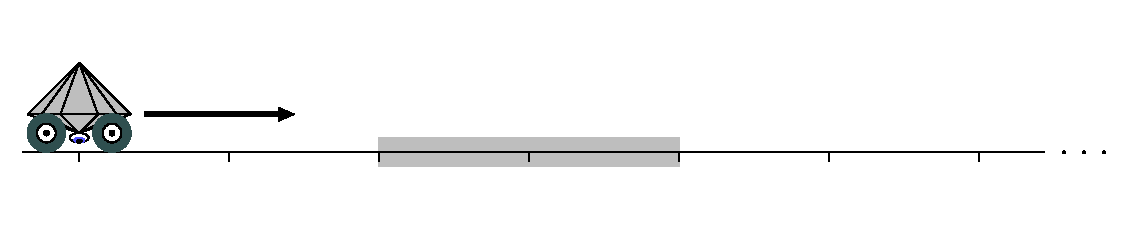
\includegraphics[width=7.5\unitlength]{Robot}}
      \newcounter{Xordinate}
      \multiput(0,0)(1,0){7}{%
        \makebox(1,0.5){$\arabic{Xordinate}$%
          \stepcounter{Xordinate}}}
      \put(2.8,0.6){\makebox(2,0.5){goal}}
    \end{picture}
  \end{center}
%\end{figure}

An intuitive way to specify the robot's behaviour is with this
\emph{knowledge-based program} (KBP), using the syntax of Dijkstra's
guarded commands:
\begin{center}
  \begin{tabular}{lll}
    $\mathbf{do}$\\
     & $\gcalt$ $\mathbf{K}_{\mbox{robot}}$ goal & $\rightarrow$ Halt\\
     & $\gcalt$ $\lnot\mathbf{K}_{\mbox{robot}}$ goal & $\rightarrow$ Nothing\\
    $\mathbf{od}$\\
  \end{tabular}
\end{center}
Here ``$\mathbf{K}_{\mbox{robot}}$ goal'' intuitively denotes ``the
robot knows it is in the goal region''
\cite[Example~7.2.2]{FHMV:1995}. We will make this precise in
\S\ref{sec:kbps-theory-kbps-semantics}, but for now note that what the
robot knows depends on the rest of the scenario, which in general may
involve other agents also running KBPs. In a sense a KBP is a very
literal rendition of a venerable artificial intelligence trope, that
what an agent does should depend on its knowledge, and what an agent
knows depends on what it does. It has been argued elsewhere
\cite{DBLP:conf/lpar/BickfordCHP04,EvdMM2000:FOSSACS,FHMV:1995} that
this is a useful level of abstraction at which to reason about
distributed systems, and some kinds of multi-agent systems
\cite{Shoham:2008}. The cost is that these specifications are not
directly executable, and it may take significant effort to find a
concrete program that has the required behaviour.

The robot does have a simple implementation however: it should halt
iff the sensor reads at least 3. That this is correct can be shown by
an epistemic model checker such as MCK \cite{DBLP:conf/cav/GammieM04}
or pencil-and-paper refinement \cite{EvdMM2000:FOSSACS}. In contrast
the goal of this work is to algorithmically discover such
implementations, which is a step towards making the work of van der
Meyden \cite{Ron:1996} practical.

The contributions of this work are as follows:
\S\ref{sec:kbps-logic-of-knowledge} develops enough of the theory of
KBPs in Isabelle/HOL \cite{Nipkow-Paulson-Wenzel:2002} to support a
formal proof of the possibility of their implementation by
finite-state automata (\S\ref{sec:kbps-automata-synthesis}). The later
sections extend this development with a full top-down derivation of an
original algorithm that constructs these implementations
(\S\ref{sec:kbps-alg}) and two instances of it
(\S\ref{sec:kbps-spr-single-agent} and
\S\ref{sec:kbps-broadcast-envs}), culminating in the mechanical
synthesis of two standard examples from the literature: the
aforementioned robot (\S\ref{sec:robot}) and the muddy children
(\S\ref{sec:mc}).

We make judicious use of parametric polymorphism and Isabelle's locale
mechanism \cite{DBLP:conf/mkm/Ballarin06} to establish and instantiate
this theory in a top-down style. Isabelle's code generator
\cite{Haftmann-Nipkow:2010:code} allows the algorithm developed here
to be directly executed on the two examples, showing that the theory
is both sound and usable. The complete development, available from the
Archive of Formal Proofs \cite{Gammie:2011}, includes the full formal
details of all claims made in this paper.

In the following we adopt the Isabelle convention of using an
apostrophe to prefix fixed but unknown types, such as
\isa{{\isacharprime}a}, and postfix type constructors
as in \isa{{\isacharprime}a\ \isafun{list}}. Other
non-standard syntax will be explained as it arises.

% We don't use "session.tex" as it includes all the dependencies.
\input{Kripke}
\input{KBPs}
\input{KBPsAuto}
\input{DFS}
\input{MapOps}
\input{KBPsAlg}

\input{Views}

\input{ClockView}

\input{SPRView}
\input{SPRViewSingle}
\input{SPRViewDet}
\input{SPRViewNonDet}
\input{SPRViewNonDetIndInit}

%%%%%%%%%%%%%%%%%%%%%%%%%%%%%%%%%%%%%%%%

\section{Examples}
\label{sec:kbps-theory-examples}

We demonstrate the theory by using Isabelle's code generator to run it
on two standard examples: the Robot from \S\ref{sec:kbps-robot-intro},
and the classic muddy children puzzle.

\input{Robot}
\input{MuddyChildren}

\section{Perspective and related work}
\label{sec:perspective}
\label{sec:kbps-alg-reduction}

The most challenging and time-consuming aspect of mechanising this
theory was making definitions suitable for the code generator. For
example, we could have used a locale to model the interface to the
maps in \S\ref{sec:kbps-alg}, but as as the code generator presently
does not cope with functions arising from locale interpretation, we
are forced to say things at least twice if we try to use both
features, as we implicitly did in \S\ref{sec:kbps-alg}. Whether it is
more convenient or even necessary to use a record and predicate or a
locale presently requires experimentation and guidance from
experienced users.

As reflected by the traffic on the Isabelle mailing list, a common
stumbling block when using the code generator is the treatment of
sets. The existing libraries are insufficiently general: Florian
Haftmann's \emph{Cset} theory\footnote{The theory \emph{Cset}
  accompanies the Isabelle/HOL distribution.} does not readily support
a choice operator, such as the one we used in \S\ref{def:choice}. Even
the heroics of the Isabelle Collections Framework
\cite{DBLP:conf/itp/LammichL10} are insufficient as there equality on
keys is structural (i.e., HOL equality), forcing us to either use a
canonical representation (such as ordered distinct lists) or redo the
relevant proofs with reified operations (equality, orderings,
etc.). Neither of these is satisfying from the perspective of reuse.

Working with suitably general theories, e.g., using data refinement,
is difficult as the simplifier is significantly less helpful for
reasoning under abstract quotients, such as those in
\S\ref{sec:kbps-alg}; what could typically be shown by equational
rewriting now involves reasoning about existentials.  For this reason
we have only allowed some types to be refined; the representations of
observations and system states are constant throughout our
development, which may preclude some optimisations. The recent work of
Kaliszyk and Urban \cite{Quotients:2011} addresses these issues for
concrete quotients, but not for the abstract ones that arise in this
kind of top-down development.

As for the use of knowledge in formally reasoning about systems, this
and similar semantics are under increasing scrutiny due to their
relation to security properties. Despite the explosion in number of
epistemic model checkers
\cite{vanEijck:DEMO:2005,DBLP:conf/cav/GammieM04,DBLP:journals/fuin/KacprzakNNPPSWZ08,DBLP:conf/cav/LomuscioQR09},
finding implementations of knowledge-based programs remains a
substantially manual affair \cite{Ron:2010}. A refinement framework
has also been developed
\cite{DBLP:conf/lpar/BickfordCHP04,EvdMM2000:FOSSACS}.

The theory presented here supports a more efficient implementation
using symbolic techniques, ala MCK; recasting the operations of the
\isafun{SimEnvironment} locale into boolean decision diagrams is
straightforward. It is readily generalised to other synchronous views,
as alluded to in \S\ref{sec:kbps-spr-single-agent}, and adding a
common knowledge modality, useful for talking about consensus
\cite[Chapter~6]{FHMV:1995}, is routine. We hope that such an
implementation will lead to more exploration of the KBP formalism.

\section{Acknowledgements}

Thanks to Kai Engelhardt for general discussions and for his
autonomous robot graphic. Florian Haftmann provided much advice on
using Isabelle/HOL's code generator and Andreas Lochbihler illuminated
the darker corners of the locale mechanism. The implementation of
Hopcroft's algorithm is due to Gerwin Klein. I am grateful to David
Greenaway, Gerwin Klein, Toby Murray and Bernie Pope for their helpful
comments.

This work was completed while I was employed by the L4.verified
project at NICTA. NICTA is funded by the Australian Government as
represented by the Department of Broadband, Communications and the
Digital Economy and the Australian Research Council through the IT
Centre of Excellence program.

\bibliographystyle{plainnat}
\bibliography{root}

\end{document}

%%% Local Variables:
%%% mode: latex
%%% TeX-master: t
%%% End:
